\documentclass{beamer}
\usepackage{csquotes}
\usepackage{tikz}
\usetikzlibrary{arrows,positioning,shapes.geometric, calc}
\usepackage{amsmath}
\usepackage{listings, xcolor}
\usepackage{lmodern}
\usepackage{adjustbox}
\usepackage{booktabs}
\usepackage{colortbl}
\usepackage{caption}
\usepackage{icomma}
\usepackage{bigstrut}
\usepackage{geometry}
\usepackage{subfigure}

\DeclareMathOperator*{\argmin}{argmin}

\usetheme{metropolis}           % Use metropolis theme
\title{Penalized Regression for predicting trait from genotypes}
\date{\today}
\author{Robert M. Porsch}
\institute{Center of Genomic Science}
\begin{document}
\maketitle

\begin{frame}[t]{Introduction}
  Our goal is to use raw genotypes to predict traits and compare it to PGS\@.
  \begin{enumerate}[(i)]
    \item Application of penalized regressions (linear models)
      \begin{itemize}
        \item $L_1$, $L_2$, and $L_0$ norm
      \end{itemize}
    \item Application of non-linear frameworks
      \begin{itemize}
        \item Neural Networks, SVM
      \end{itemize}
  \end{enumerate}
  Identify and estimate epistatic effects.
\end{frame}

\section{Simple Simulation}
\label{sec:simulation}

\begin{frame}[t]{Some simple simulation}
  I simulated some toy data with $n = 10,000$ with $p = 10,000$. 
  Effect sizes of 1\% of variables were drawn from a $\mathcal{N}(0, 0.01)$, the rest are set to 0.

  \begin{figure}[htpb]
    \centering
    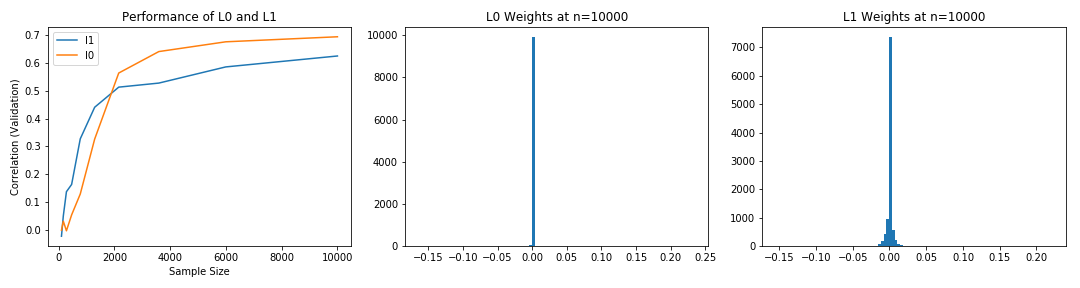
\includegraphics[width=0.99\linewidth]{./performance.png}
  \end{figure}
  \begin{columns}
    \begin{column}{0.35\textwidth}
      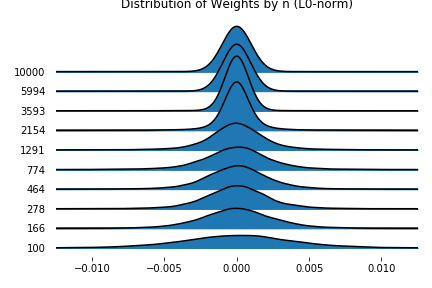
\includegraphics[width=0.99\linewidth]{./joyplot_l0.png}
    \end{column}
    \begin{column}{0.35\textwidth}
      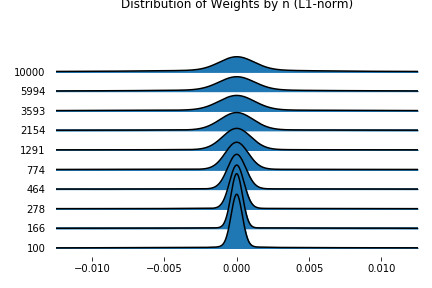
\includegraphics[width=0.99\linewidth]{./joyplot_l1.png}
    \end{column}
    \begin{column}{0.35\textwidth}
      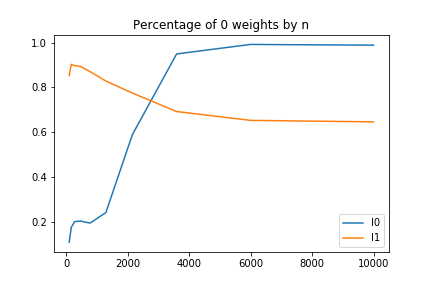
\includegraphics[width=0.99\linewidth]{./percentage_0_l0l1.png}
    \end{column}
  \end{columns}
\end{frame}

\begin{frame}[t]{}
  \begin{figure}[htpb]
    \centering
    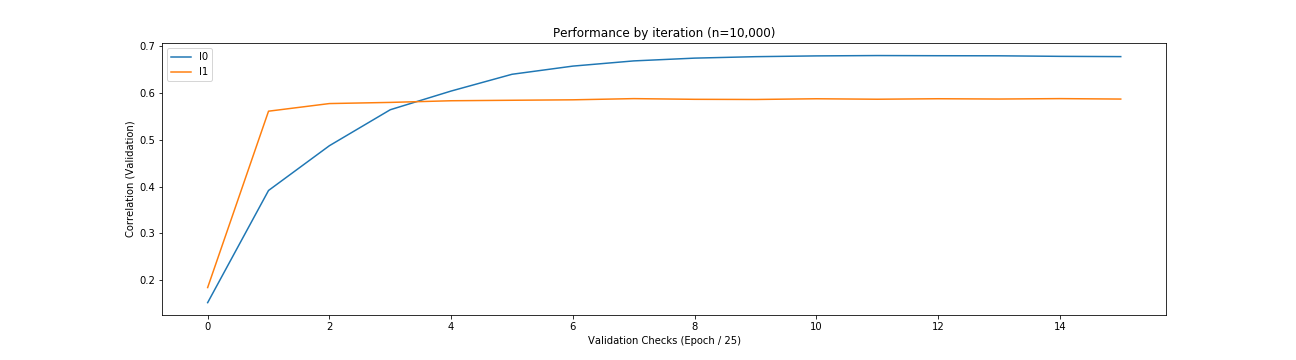
\includegraphics[width=0.999\linewidth]{./performance_epochs_l1l0.png} \\
  \end{figure}
  \begin{figure}[htpb]
    \centering
    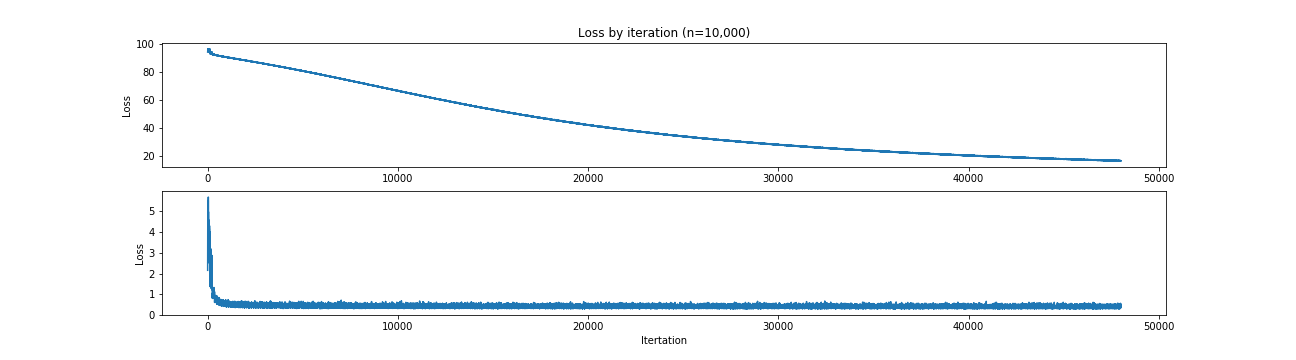
\includegraphics[width=0.999\linewidth]{./loss_l1l0.png} \\
  \end{figure}
\end{frame}

\section{Combing $L_0$ and $L0_1$}
\label{sec:combing_l_0_and_l0_1_}

\begin{frame}[t]{Connection between the $L_2$-norm and Gaussian prior}
  \small
  Let $\mathcal{D}$ the dataset consisting of $N$ input-output pairs $\{(x_1, y_1), \ldots, (x_N, y_N)\}$.

  Lets also assume that the output is linear related via $\theta$ and that the data is corrupted by some noise $\epsilon\sim N(0, \sigma^2)$.
  Then the Gaussian likelihood is:
  \begin{equation}
    \prod^N_{i=1} \mathcal{N}(y_i|\theta x_i, \sigma^2)
  \end{equation}
  We can then impose a Gaussian prior $\mathcal{N}(\theta|0, \lambda^{-1})$, in which $\lambda$ is a positive scalar.
  Then we have for the likelihood:
  \begin{equation}
    \prod^N_{i=1} \mathcal{N}(y_i|\theta x_i, \sigma^2)\mathcal{N}(\theta|0, \lambda^{-1})
  \end{equation}
  Taking the logarithm of the above and removing unecessary constants we get:
  \begin{equation}
    \sum^N_{i=1} - \frac{1}{\sigma^2} (y_i - \theta x_i)^2 - \lambda \theta^2 + const.
  \end{equation}
\end{frame}

\begin{frame}[t]{Combining $L_0$ and $L_2$}
  \small
  Often it is desirable to shrink paramenters, hence on should combine $L_0$ and other norms.
  Using the $L_2$-norm and under a bernulli gating mechanism:
  \begin{equation}
    \mathbb{E}_{q(z|\pi)} [||\theta||^2_2] = \sum^P_{j=1} \mathbb{E}_{q(z_j|\pi_j)} [z_j^2\tilde{\theta}^2_j] = \sum^P_{j=1} \pi_j \tilde{\theta}^2_j
  \end{equation}
  in which $\pi_j$ is the probability of the gate being open.

  Since the $L_2$ norm is proportional to the negative log density of $\mathcal{N}(0, \sigma^2)$ we can assume that the $\sigma$ for each $\theta$ is controlled by $z$.
  That is if $z=0 \rightarrow \sigma=1$, while if $z > 0 \rightarrow \sigma = z$
  Hence the $L_2$ norm is then (where $\hat{\theta} = \frac{\theta}{\sigma}$)
  \begin{equation}
    \begin{split}
      \mathbb{E}_{q(z|\pi)} [||\hat{\theta}||^2_2] =  & \sum^P_{j=1} (1 - Q_{\hat{s}_j}(0 | \phi_j)) \mathbb{E}_{q(z_j|\pi_j, \hat{s}_j > 0)} [\frac{\tilde{\theta}^2_j z^2_j}{z^2_j}] \\
                                                & \sum^P_{j=1} (1 - Q_{\hat{s}_j}(0 | \phi_j)) \tilde{\theta}^2_j
      \end{split}
  \end{equation}
\end{frame}

\begin{frame}[t]{Results of $L_{0,2}$}
  
\end{frame}

\begin{frame}[t]{Simulation Framework}
  \begin{center}
  \textbf{Completely blind. You need to ask Tim.}
  \end{center}
  \\
  But here is what I know:
  \begin{itemize}
    \item Linear and non-linear effects present
    \item Currently only using chromosome 10
    \item $R^2$ between $0.04$ and $0.01$
    \item Performance of Lassosum is a correlation of $0.05$
  \end{itemize}
\end{frame}

\begin{frame}[t]{Task processing}
  \begin{figure}[htpb]
    \centering
    \includegraphics[width=0.8\linewidth]{Dask_processing.png}
  \end{figure} 
\end{frame}

\begin{frame}[t]{Some Results}
  \begin{figure}[htpb]
    \centering
    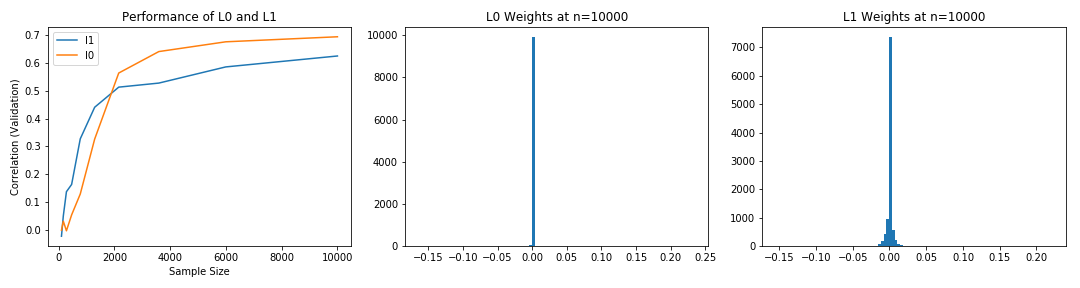
\includegraphics[width=0.99\linewidth]{performance.png}
    \caption{Performance}
  \end{figure}
\end{frame}

\begin{frame}[t]{Parameter Space}
  \begin{figure}[htpb]
    \centering
    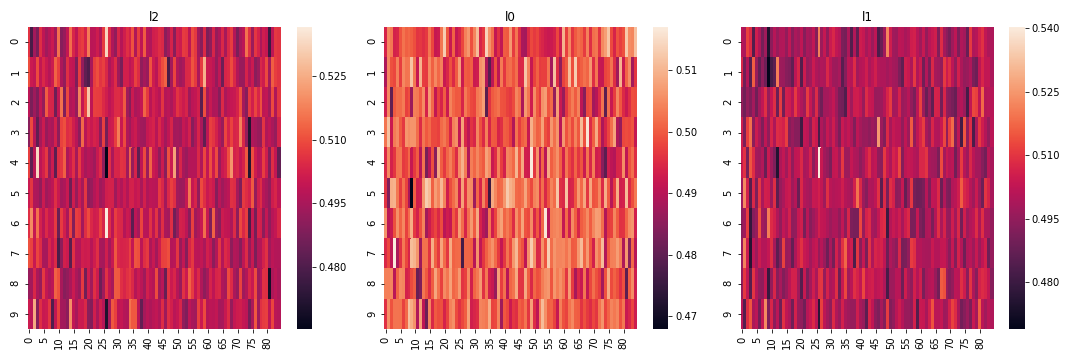
\includegraphics[width=0.99\linewidth]{null_proportion.png}
    \caption{Proportion of parameters equal or close to 0}
  \end{figure}
  \begin{itemize}
    \item $L_0$ comes very quickly to sparse solution (parameters are not accurate, small effects)
    \item $L_1$ and $L_2$ seem to take a bit longer
  \end{itemize}
\end{frame}

\section{Suplementary for $L_0$-norm}
\label{sec:suplementary}

\begin{frame}[t]{Penalized Regression}
  Let $\mathcal{D}$ the dataset consisting of $N$ input-output pairs $\{(x_1, y_1), \ldots, (x_N, y_N)\}$ and consider the following regularized minimization procedure

  \begin{equation} 
    \mathcal{R}(\theta) = \frac{1}{N} ( \sum^N_{i=1} \mathcal{L}(h(x_i; \theta), y_i)) + \lambda\mathcal{P}(\theta)
  \end{equation}

  With $\theta^* = \underset{\theta}{\argmin}\{\mathcal{R}(\theta)\}$.

  $\mathcal{P}(\theta)$ is a penalization function for the parameters $\theta$.
\end{frame}

\begin{frame}[t]{The General Recipe}
  The first step is to reformulate the $L_0$ norm under the parameters $\theta$.
  Hence let,
  \begin{equation}
    \begin{matrix}
      \theta_j = \tilde{\theta_j}z_j, & z_j \in \{0, 1\}, & \tilde{\theta}_j \neq 0
    \end{matrix}
  \end{equation}
  Therefore $z_j$ can be considered as binary gates (parameter has an effect).

  Then we can reformulate the minimization from Eq. 1 by letting $q(z_j|\pi_j) = Bern(\pi_j)$
  \begin{equation}
    \mathcal{R}(\tilde{\theta}, \pi) = \mathbb{E}_{q(z|\pi)} [\frac{1}{N} ( \sum^N_{i=1} \mathcal{L}(h(x_i; \tilde{\theta} \otimes z), y_i)] + \lambda \sum^{p}_{j=1} \pi_j
  \end{equation}
  with  $\tilde{\theta}^*, \pi^* = \underset{{\tilde{\theta}, \pi}}{\argmin} \{\mathcal{R}(\tilde{\theta}, \pi)\}$

  However, the discrete nature of $z$ makes it still difficult to minimize $\pi$.
\end{frame}

\begin{frame}[t]{Hard-sigmoid function}
  \small
  Let s be a continuous random variable with a distribution $q(s)$ with parameter $\phi$.
  Then we can give the gates $z$ a hard sigmoid function with:
  \begin{equation}
    \begin{align*}
      s \sim& q(s|\phi) \\
      z =& \min(1, \max(0, s))
    \end{align*}
  \end{equation}
  Then the probability of the gates being non-zero is
  \begin{equation}
    q(z \neq 0 | \delata) =  1 - Q(s\leq 0 | \phi)
  \end{equation}
  in which $Q(\cdot)$ is the cumulative distribution function of s
  \begin{equation}
    \begin{split}
      \mathcal{R}(\tilde{\theta}, \phi) = \mathbb{E}_{q(s|\phi)} [\frac{1}{N} ( \sum^N_{i=1} \mathcal{L}(h(x_i; \tilde{\theta} \otimes g(s)), y_i)] + \\ 
      \lambda \sum^{|\theta|}_{j=1} (1 - Q(s_j \leq 0 | \phi_j))
    \end{split}
  \end{equation}
  with $\theta^*, \phi^* = \underset{{\tilde{\theta}, \phi}}{\argmin} \{\mathcal{R}(\tilde{\theta}, \phi)\}$ and $g(\cdot) = \min(1, \max(0, \cdot))$
\end{frame}


\begin{frame}[t]{The Hard Concrete Distribution}
  The literature suggests to use a hard concrete distribution as a smoothing function $q(s)$. 
  The parameters of the distribution are $\phi = (\log \alpha, \beta)$ and can be stretched to $(\gamma, \zeta)$ intervals.
  \begin{equation}
    \begin{align*}
      u \sim \mathcal{U}(0,1) \\
      s = Sigmoid((\log u - \log(1-u) + \log\alpha)/\beta) \\
      \bar{s} = s(\zeta - \gamma) + \gamma 
    \end{align*}
  \end{equation}
  \begin{figure}[htpb]
    \centering
    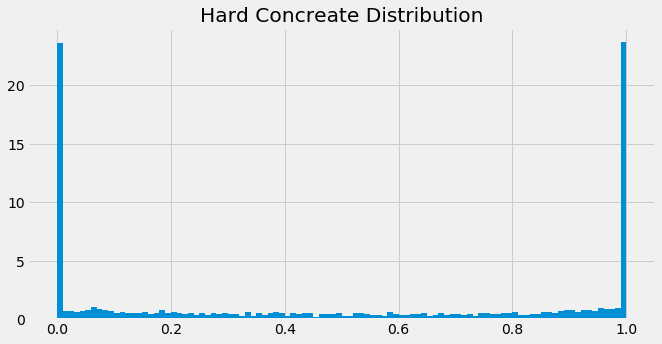
\includegraphics[width=0.5\linewidth]{hard_concrete.png}
    \caption{Sample from the Hard Concrete Distribution}\label{fig:hard_concrete}
  \end{figure} 
\end{frame}

\begin{frame}[t]{Connection between the $L_2$-norm and Gaussian prior}
  \small
  Let $\mathcal{D}$ the dataset consisting of $N$ input-output pairs $\{(x_1, y_1), \ldots, (x_N, y_N)\}$.

  Lets also assume that the output is linear related via $\theta$ and that the data is corrupted by some noise $\epsilon\sim N(0, \sigma^2)$.
  Then the Gaussian likelihood is:
  \begin{equation}
    \prod^N_{i=1} \mathcal{N}(y_i|\theta x_i, \sigma^2)
  \end{equation}
  We can then impose a Gaussian prior $\mathcal{N}(\theta|0, \lambda^{-1})$, in which $\lambda$ is a positive scalar.
  Then we have for the likelihood:
  \begin{equation}
    \prod^N_{i=1} \mathcal{N}(y_i|\theta x_i, \sigma^2)\mathcal{N}(\theta|0, \lambda^{-1})
  \end{equation}
  Taking the logarithm of the above and removing unecessary constants we get:
  \begin{equation}
    \sum^N_{i=1} - \frac{1}{\sigma^2} (y_i - \theta x_i)^2 - \lambda \theta^2 + const.
  \end{equation}
\end{frame}

\begin{frame}[t]{Combining $L_0$ and $L_2$}
  \small
  Often it is desirable to shrink paramenters, hence on should combine $L_0$ and other norms.
  
  Using the $L_2$-norm and under a bernulli gating mechanism:
  \begin{equation}
    \mathbb{E}_{q(z|\pi)} [||\theta||^2_2] = \sum^P_{j=1} \mathbb{E}_{q(z_j|\pi_j)} [z_j^2\tilde{\theta}^2_j] = \sum^P_{j=1} \pi_j \tilde{\theta}^2_j
  \end{equation}
  in which $\pi_j$ is the probability of the gate being open.

  Since the $L_2$ norm is proportional to the negative log density of $\mathcal{N}(0, \sigma^2)$ we can assume that the $\sigma$ for each $\theta$ is controlled by $z$.
  That is if $z=0 \rightarrow \sigma=1$, while if $z > 0 \rightarrow \sigma = z$
  Hence the $L_2$ norm is then (where $\hat{\theta} = \frac{\theta}{\sigma}$)
  \begin{equation}
    \begin{split}
      \mathbb{E}_{q(z|\pi)} [||\hat{\theta}||^2_2] =  & \sum^P_{j=1} (1 - Q_{\hat{s}_j}(0 | \phi_j)) \mathbb{E}_{q(z_j|\pi_j, \hat{s}_j > 0)} [\frac{\tilde{\theta}^2_j z^2_j}{z^2_j}] \\
                                                & \sum^P_{j=1} (1 - Q_{\hat{s}_j}(0 | \phi_j)) \tilde{\theta}^2_j
      \end{split}
  \end{equation}
  
\end{frame}

\begin{frame}[t]{Challenges}
  \textbf{Challenge:} \\
  The plumbing (data engineering)
  \\
  \begin{itemize}
    \item Process of the UKB in parallel efficiently
    \item Large Memory requirements for the UKB (scaling)
    \item Currently using Dask on our cluster
  \end{itemize}
  The optimization/implementation:
  \begin{itemize}
    \item Works fine on test data (1k Genome Project)
    \item Issues with larger data
    \item size of mini-batch size
    \item choosing appropriate learning rates
  \end{itemize}
\end{frame}


\end{document}
